\begin{frame}[t]{Hohe ACC}
		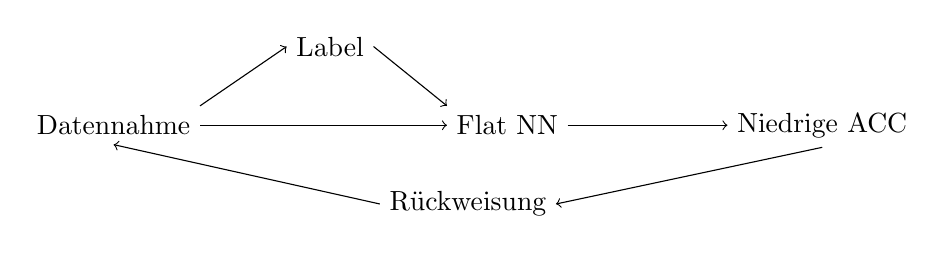
\begin{tikzpicture}[node distance=4cm]
				\node (A) {Datennahme};
				\node (B) [right of=A, xshift=-1.25cm, yshift=1cm] {Label};
				\node (C) [right of=A, xshift=1cm] {Flat NN};
				\node (D) [right of=C] {Niedrige ACC};
				\node (E) [below of=C, yshift=3cm, xshift=-0.5cm] {Rückweisung};

				\draw [->, right of=A] (A.north east) -- (B.west);
				\draw [->] (B.east) -- (C.north west);
				\draw [->] (A) -- (C);
				\draw [->] (C) -- (D);
				\draw [->] (D.south) -- (E.east);
				\draw [->] (E.west) -- (A.south);
		\end{tikzpicture}
\end{frame}
